\documentclass[11pt, a4paper, fleqn]{article}
\usepackage[utf8]{inputenc}
\usepackage{amsmath}
\usepackage{amsfonts}
\usepackage{hyperref}
\usepackage{amssymb}
\usepackage{subcaption}
\usepackage{amsthm}
\usepackage{graphicx}
\usepackage{mdframed}
\usepackage{bigints}
\usepackage{verbatim}
\usepackage{bbm}
\usepackage{cancel}
\usepackage[ruled]{algorithm2e}
\usepackage[left=1in,right=1in,top=1in,bottom=1in]{geometry}
\usepackage{enumitem,xparse}
\newtheorem{theorem}{Theorem}[section]
\newtheorem{corollary}{Corollary}[theorem]
\newtheorem{lemma}[theorem]{Lemma}
\ExplSyntaxOn
\DeclareExpandableDocumentCommand \AlphToNum { m }
{
   \int_from_alph:n { #1 }
}
\ExplSyntaxOff

\let\normalint\int % PS
\def\int{\displaystyle\normalint} %PS

\newenvironment{enumeratei}{\begin{enumerate}[\upshape (i)]}{\end{enumerate}}
\newenvironment{enumeratea}{\begin{enumerate}[\upshape (a)]}{\end{enumerate}}
\newenvironment{enumeraten}{\begin{enumerate}[\upshape 1.]}{\end{enumerate}}
\newenvironment{enumerateA}{\begin{enumerate}[\upshape (A)]}{\end{enumerate}}

\numberwithin{equation}{section}
\numberwithin{figure}{section}
\numberwithin{table}{section}
%%%%%%%%%%%%%%%%%%%%%%%%%%%%%%%%%%%%%%%%%%%    
%% Local environments 
\newtheorem{thm}{Theorem}[section]
\newtheorem{lem}[thm]{Lemma}
\newtheorem{cor}[thm]{Corollary}
\newtheorem{prop}[thm]{Proposition}
\newtheorem{defn}[thm]{Definition}
\newtheorem{rem}[thm]{Remark}
\newtheorem{hyp}[thm]{Hypothesis}
\newtheorem{ass}[thm]{Assumption}
\newtheorem{exc}[section]{Exercise}
\newtheorem{ex}[thm]{Example}
\newtheorem{conj}[thm]{Conjecture}   
%%%%%%%%%%%%%%%%%%%%%%%%%%%%%%%%%%%%%%%%%%%
%% Local macros
\renewcommand{\leq}{\leqslant} 
\renewcommand{\geq}{\geqslant} 
\newcommand{\eset}{\varnothing}
\newcommand{\ra}{\rangle}
\newcommand{\la}{\langle} 
\newcommand{\wt}{\widetilde}
\newcommand{\pms}{\{-1,1\}}
\newcommand{\ind}{\mathds{1}}
\newcommand{\eps}{\varepsilon}
\newcommand{\To}{\longrightarrow}
\newcommand{\norm}[1]{\left\Vert#1\right\Vert}
\newcommand{\abs}[1]{\left\vert#1\right\vert}
\newcommand{\set}[1]{\left\{#1\right\}}
\newcommand{\goesto}{\longrightarrow}
\newcommand{\Real}{\mathds{R}}
\newcommand{\Complex}{\mathds{C}}
\newcommand{\ie}{\emph{i.e.,}}
\newcommand{\as}{\emph{a.e.}}
\newcommand{\eg}{\emph{e.g.,}}
\renewcommand{\iff}{\Leftrightarrow} 
\newcommand{\equald}{\stackrel{\mathrm{d}}{=}}
\newcommand{\probc}{\stackrel{\mathrm{P}}{\longrightarrow}}
\newcommand{\probd}{\stackrel{\mathrm{d}}{\Longrightarrow}}
\newcommand{\weakc}{\stackrel{\mathrm{w}}{\longrightarrow}}
\newcommand{\fpar}[2]{\frac{\partial #1}{\partial #2}}
\newcommand{\spar}[2]{\frac{\partial^2 #1}{\partial #2^2}}
\newcommand{\mpar}[3]{\frac{\partial^2 #1}{\partial #2 \partial #3}}  
\def\qed{ \hfill $\blacksquare$}  
%%%%%%%%%%%%%%%%%%%%%%%%%%%%%%%%%%%%%%%%%%%
%% Greek symbols
\let\ga=\alpha \let\gb=\beta \let\gc=\gamma \let\gd=\delta \let\gee=\epsilon
\let\gf=\varphi \let\gh=\eta \let\gi=\iota  \let\gk=\kappa \let\gl=\lambda \let\gm=\mu      
\let\gn=\nu \let\go=\omega \let\gp=\pi \let\gr=\rho \let\gs=\sigma \let\gt=\tau \let\gth=\vartheta
\let\gx=\chi \let\gy=\upsilon \let\gz=\zeta
\let\gC=\Gamma \let\gD=\Delta \let\gF=\Phi \let\gL=\Lambda \let\gTh=\Theta
\let\gO=\Omega   \let\gP=\Pi    \let\gPs=\Psi  \let\gS=\Sigma \let\gU=\Upsilon \let\gX=\Chi
\let\gY=\Upsilon                                
%%%%%%%%%%%%%%%%%%%%%%%%%%%%%%%%%%%%%%%%%%%
%% MathCal symbols
\newcommand{\mc}[1]{\mathcal{#1}}
\newcommand{\cA}{\mathcal{A}}\newcommand{\cB}{\mathcal{B}}\newcommand{\cC}{\mathcal{C}}
\newcommand{\cD}{\mathcal{D}}\newcommand{\cE}{\mathcal{E}}\newcommand{\cF}{\mathcal{F}}
\newcommand{\cG}{\mathcal{G}}\newcommand{\cH}{\mathcal{H}}\newcommand{\cI}{\mathcal{I}}
\newcommand{\cJ}{\mathcal{J}}\newcommand{\cK}{\mathcal{K}}\newcommand{\cL}{\mathcal{L}}
\newcommand{\cM}{\mathcal{M}}\newcommand{\cN}{\mathcal{N}}\newcommand{\cO}{\mathcal{O}}
\newcommand{\cP}{\mathcal{P}}\newcommand{\cQ}{\mathcal{Q}}\newcommand{\cR}{\mathcal{R}}
\newcommand{\cS}{\mathcal{S}}\newcommand{\cT}{\mathcal{T}}\newcommand{\cU}{\mathcal{U}}
\newcommand{\cV}{\mathcal{V}}\newcommand{\cW}{\mathcal{W}}\newcommand{\cX}{\mathcal{X}}
\newcommand{\cY}{\mathcal{Y}}\newcommand{\cZ}{\mathcal{Z}}  
%%%%%%%%%%%%%%%%%%%%%%%%%%%%%%%%%%%%%%%%%%%
%% Math Boldface Symbols
\newcommand{\vzero}{\mathbf{0}}\newcommand{\vone}{\mathbf{1}}\newcommand{\vtwo}{\mathbf{2}}
\newcommand{\vthree}{\mathbf{3}}\newcommand{\vfour}{\mathbf{4}}\newcommand{\vfive}{\mathbf{5}}
\newcommand{\vsix}{\mathbf{6}}\newcommand{\vseven}{\mathbf{7}}\newcommand{\veight}{\mathbf{8}}
\newcommand{\vnine}{\mathbf{9}}\newcommand{\vA}{\mathbf{A}}\newcommand{\vB}{\mathbf{B}}
\newcommand{\vC}{\mathbf{C}}\newcommand{\vD}{\mathbf{D}}\newcommand{\vE}{\mathbf{E}}
\newcommand{\vF}{\mathbf{F}}\newcommand{\vG}{\mathbf{G}}\newcommand{\vH}{\mathbf{H}}
\newcommand{\vI}{\mathbf{I}}\newcommand{\vJ}{\mathbf{J}}\newcommand{\vK}{\mathbf{K}}
\newcommand{\vL}{\mathbf{L}}\newcommand{\vM}{\mathbf{M}}\newcommand{\vN}{\mathbf{N}}
\newcommand{\vO}{\mathbf{O}}\newcommand{\vP}{\mathbf{P}}\newcommand{\vQ}{\mathbf{Q}}
\newcommand{\vR}{\mathbf{R}}\newcommand{\vS}{\mathbf{S}}\newcommand{\vT}{\mathbf{T}}
\newcommand{\vU}{\mathbf{U}}\newcommand{\vV}{\mathbf{V}}\newcommand{\vW}{\mathbf{W}}
\newcommand{\vX}{\mathbf{X}}\newcommand{\vY}{\mathbf{Y}}\newcommand{\vZ}{\mathbf{Z}}
\newcommand{\va}{\mathbf{a}}\newcommand{\vb}{\mathbf{b}}\newcommand{\vc}{\mathbf{c}}
\newcommand{\vd}{\mathbf{d}}\newcommand{\ve}{\mathbf{e}}\newcommand{\vf}{\mathbf{f}}
\newcommand{\vg}{\mathbf{g}}\newcommand{\vh}{\mathbf{h}}\newcommand{\vi}{\mathbf{i}}
\newcommand{\vj}{\mathbf{j}}\newcommand{\vk}{\mathbf{k}}\newcommand{\vl}{\mathbf{l}}
\newcommand{\vm}{\mathbf{m}}\newcommand{\vn}{\mathbf{n}}\newcommand{\vo}{\mathbf{o}}
\newcommand{\vp}{\mathbf{p}}\newcommand{\vq}{\mathbf{q}}\newcommand{\vr}{\mathbf{r}}
\newcommand{\vs}{\mathbf{s}}\newcommand{\vt}{\mathbf{t}}\newcommand{\vu}{\mathbf{u}}
\newcommand{\vv}{\mathbf{v}}\newcommand{\vw}{\mathbf{w}}\newcommand{\vx}{\mathbf{x}}
\newcommand{\vy}{\mathbf{y}}\newcommand{\vz}{\mathbf{z}} 
%%%%%%%%%%%%%%%%%%%%%%%%%%%%%%%%%%%%%%%%%%%  
%% Math Bold Symbols commands  
\newcommand{\mv}[1]{\boldsymbol{#1}}\newcommand{\mvinfty}{\boldsymbol{\infty}}\newcommand{\mvzero}{\boldsymbol{0}}
\newcommand{\mvone}{\boldsymbol{1}}\newcommand{\mvtwo}{\boldsymbol{2}}\newcommand{\mvthree}{\boldsymbol{3}}
\newcommand{\mvfour}{\boldsymbol{4}}\newcommand{\mvfive}{\boldsymbol{5}}\newcommand{\mvsix}{\boldsymbol{6}}
\newcommand{\mvseven}{\boldsymbol{7}}\newcommand{\mveight}{\boldsymbol{8}}\newcommand{\mvnine}{\boldsymbol{9}}
\newcommand{\mvA}{\boldsymbol{A}}\newcommand{\mvB}{\boldsymbol{B}}\newcommand{\mvC}{\boldsymbol{C}}
\newcommand{\mvD}{\boldsymbol{D}}\newcommand{\mvE}{\boldsymbol{E}}\newcommand{\mvF}{\boldsymbol{F}}
\newcommand{\mvG}{\boldsymbol{G}}\newcommand{\mvH}{\boldsymbol{H}}\newcommand{\mvI}{\boldsymbol{I}}
\newcommand{\mvJ}{\boldsymbol{J}}\newcommand{\mvK}{\boldsymbol{K}}\newcommand{\mvL}{\boldsymbol{L}}
\newcommand{\mvM}{\boldsymbol{M}}\newcommand{\mvN}{\boldsymbol{N}}\newcommand{\mvO}{\boldsymbol{O}}
\newcommand{\mvP}{\boldsymbol{P}}\newcommand{\mvQ}{\boldsymbol{Q}}\newcommand{\mvR}{\boldsymbol{R}}
\newcommand{\mvS}{\boldsymbol{S}}\newcommand{\mvT}{\boldsymbol{T}}\newcommand{\mvU}{\boldsymbol{U}}
\newcommand{\mvV}{\boldsymbol{V}}\newcommand{\mvW}{\boldsymbol{W}}\newcommand{\mvX}{\boldsymbol{X}}
\newcommand{\mvY}{\boldsymbol{Y}}\newcommand{\mvZ}{\boldsymbol{Z}}\newcommand{\mva}{\boldsymbol{a}}
\newcommand{\mvb}{\boldsymbol{b}}\newcommand{\mvc}{\boldsymbol{c}}\newcommand{\mvd}{\boldsymbol{d}}
\newcommand{\mve}{\boldsymbol{e}}\newcommand{\mvf}{\boldsymbol{f}}\newcommand{\mvg}{\boldsymbol{g}}
\newcommand{\mvh}{\boldsymbol{h}}\newcommand{\mvi}{\boldsymbol{i}}\newcommand{\mvj}{\boldsymbol{j}}
\newcommand{\mvk}{\boldsymbol{k}}\newcommand{\mvl}{\boldsymbol{l}}\newcommand{\mvm}{\boldsymbol{m}}
\newcommand{\mvn}{\boldsymbol{n}}\newcommand{\mvo}{\boldsymbol{o}}\newcommand{\mvp}{\boldsymbol{p}}
\newcommand{\mvq}{\boldsymbol{q}}\newcommand{\mvr}{\boldsymbol{r}}\newcommand{\mvs}{\boldsymbol{s}}
\newcommand{\mvt}{\boldsymbol{t}}\newcommand{\mvu}{\boldsymbol{u}}\newcommand{\mvv}{\boldsymbol{v}}
\newcommand{\mvw}{\boldsymbol{w}}\newcommand{\mvx}{\boldsymbol{x}}\newcommand{\mvy}{\boldsymbol{y}}
\newcommand{\mvz}{\boldsymbol{z}}
\newcommand{\mvga}{\boldsymbol{\alpha}}\newcommand{\mvgb}{\boldsymbol{\beta}}\newcommand{\mvgc}{\boldsymbol{\gamma}}
\newcommand{\mvgC}{\boldsymbol{\Gamma}}\newcommand{\mvgd}{\boldsymbol{\delta}}\newcommand{\mvgD}{\boldsymbol{\Delta}}
\newcommand{\mvgee}{\boldsymbol{\epsilon}}\newcommand{\mveps}{\boldsymbol{\eps}}\newcommand{\mvgf}{\boldsymbol{\varphi}}
\newcommand{\mvgF}{\boldsymbol{\Phi}}\newcommand{\mvgth}{\boldsymbol{\theta}}\newcommand{\mvgTh}{\boldsymbol{\Theta}}
\newcommand{\mvgh}{\boldsymbol{\eta}}\newcommand{\mvgi}{\boldsymbol{\iota}}\newcommand{\mvgk}{\boldsymbol{\kappa}}
\newcommand{\mvgl}{\boldsymbol{\lambda}}\newcommand{\mvgL}{\boldsymbol{\Lambda}}\newcommand{\mvgm}{\boldsymbol{\mu}}
\newcommand{\mvgn}{\boldsymbol{\nu}}\newcommand{\mvgo}{\boldsymbol{\omega}}\newcommand{\mvgO}{\boldsymbol{\Omega}}
\newcommand{\mvgp}{\boldsymbol{\pi}}\newcommand{\mvgP}{\boldsymbol{\Pi}}\newcommand{\mvgr}{\boldsymbol{\rho}}
\newcommand{\mvgs}{\boldsymbol{\sigma}}\newcommand{\mvgS}{\boldsymbol{\Sigma}}\newcommand{\mvgt}{\boldsymbol{\tau}}
\newcommand{\mvgu}{\boldsymbol{\upsilon}}\newcommand{\mvgU}{\boldsymbol{\Upsilon}}\newcommand{\mvgx}{\boldsymbol{\chi}}
\newcommand{\mvgz}{\boldsymbol{\zeta}}\newcommand{\mvalpha}{\boldsymbol{\alpha}}\newcommand{\mvbeta}{\boldsymbol{\beta}}
\newcommand{\mvgamma}{\boldsymbol{\gamma}}\newcommand{\mvGamma}{\boldsymbol{\Gamma}}\newcommand{\mvdelta}{\boldsymbol{\delta}}
\newcommand{\mvDelta}{\boldsymbol{\Delta}}\newcommand{\mvepsilon}{\boldsymbol{\epsilon}}\newcommand{\mvphi}{\boldsymbol{\phi}}
\newcommand{\mvPhi}{\boldsymbol{\Phi}}\newcommand{\mvtheta}{\boldsymbol{\theta}}\newcommand{\mvTheta}{\boldsymbol{\Theta}}
\newcommand{\mveta}{\boldsymbol{\eta}}\newcommand{\mviota}{\boldsymbol{\iota}}\newcommand{\mvkappa}{\boldsymbol{\kappa}}
\newcommand{\mvlambda}{\boldsymbol{\lambda}}\newcommand{\mvLambda}{\boldsymbol{\Lambda}}\newcommand{\mvmu}{\boldsymbol{\mu}}
\newcommand{\mvnu}{\boldsymbol{\nu}}
\newcommand{\mvomega}{\boldsymbol{\omega}}\newcommand{\mvOmega}{\boldsymbol{\Omega}}\newcommand{\mvpi}{\boldsymbol{\pi}}
\newcommand{\mvPi}{\boldsymbol{\Pi}}\newcommand{\mvrho}{\boldsymbol{\rho}}\newcommand{\mvsigma}{\boldsymbol{\sigma}}
\newcommand{\mvSigma}{\boldsymbol{\Sigma}}\newcommand{\mvtau}{\boldsymbol{\tau}}\newcommand{\mvupsilon}{\boldsymbol{\upsilon}}
\newcommand{\mvUpsilon}{\boldsymbol{\Upsilon}}\newcommand{\mvchi}{\boldsymbol{\chi}}\newcommand{\mvzeta}{\boldsymbol{\zeta}}
\newcommand{\mvvartheta}{\boldsymbol{\vartheta}}\newcommand{\mvxi}{\boldsymbol{\xi}}\newcommand{\mvXi}{\boldsymbol{\Xi}}
\newcommand{\mvomic}{\boldsymbol{\o}}\newcommand{\mvvarpi}{\boldsymbol{\varpi}}\newcommand{\mvvarrho}{\boldsymbol{\varrho}}
\newcommand{\mvvarsigma}{\boldsymbol{\varsigma}}\newcommand{\mvvarphi}{\boldsymbol{\varphi}}\newcommand{\mvpsi}{\boldsymbol{\psi}}\newcommand{\mvPsi}{\boldsymbol{\Psi}}   
%%%%%%%%%%%%%%%%%%%%%%%%%%%%%%%%%%%%%%%%%%%
%% Math Frakur fonts except for i which is \mfi
\newcommand{\f}[1]{\mathfrak{#1}}
\newcommand{\fA}{\mathfrak{A}}\newcommand{\fB}{\mathfrak{B}}\newcommand{\fC}{\mathfrak{C}}
\newcommand{\fD}{\mathfrak{D}}\newcommand{\fE}{\mathfrak{E}}\newcommand{\fF}{\mathfrak{F}}
\newcommand{\fG}{\mathfrak{G}}\newcommand{\fH}{\mathfrak{H}}\newcommand{\fI}{\mathfrak{I}}
\newcommand{\fJ}{\mathfrak{J}}\newcommand{\fK}{\mathfrak{K}}\newcommand{\fL}{\mathfrak{L}}
\newcommand{\fM}{\mathfrak{M}}\newcommand{\fN}{\mathfrak{N}}\newcommand{\fO}{\mathfrak{O}}
\newcommand{\fP}{\mathfrak{P}}\newcommand{\fQ}{\mathfrak{Q}}\newcommand{\fR}{\mathfrak{R}}
\newcommand{\fS}{\mathfrak{S}}\newcommand{\fT}{\mathfrak{T}}\newcommand{\fU}{\mathfrak{U}}
\newcommand{\fV}{\mathfrak{V}}\newcommand{\fW}{\mathfrak{W}}\newcommand{\fX}{\mathfrak{X}}
\newcommand{\fY}{\mathfrak{Y}}\newcommand{\fZ}{\mathfrak{Z}}\newcommand{\fa}{\mathfrak{a}}
\newcommand{\fb}{\mathfrak{b}}\newcommand{\fc}{\mathfrak{c}}\newcommand{\fd}{\mathfrak{d}}
\newcommand{\fe}{\mathfrak{e}}\newcommand{\ff}{\mathfrak{f}}\newcommand{\fg}{\mathfrak{g}}
\newcommand{\fh}{\mathfrak{h}}\newcommand{\mfi}{\mathfrak{i}}\newcommand{\fj}{\mathfrak{j}}
\newcommand{\fk}{\mathfrak{k}}\newcommand{\fl}{\mathfrak{l}}\newcommand{\fm}{\mathfrak{m}}
\newcommand{\fn}{\mathfrak{n}}\newcommand{\fo}{\mathfrak{o}}\newcommand{\fp}{\mathfrak{p}}
\newcommand{\fq}{\mathfrak{q}}\newcommand{\fr}{\mathfrak{r}}\newcommand{\fs}{\mathfrak{s}}
\newcommand{\ft}{\mathfrak{t}}\newcommand{\fu}{\mathfrak{u}}\newcommand{\fv}{\mathfrak{v}}
\newcommand{\fw}{\mathfrak{w}}\newcommand{\fx}{\mathfrak{x}}\newcommand{\fy}{\mathfrak{y}}
\newcommand{\fz}{\mathfrak{z}}  
%%%%%%%%%%%%%%%%%%%%%%%%%%%%%%%%%%%%%%%%%%%
% Double capital letters
\newcommand{\bb}[1]{\mathbb{#1}}
\newcommand{\bA}{\mathbb{A}}\newcommand{\bB}{\mathbb{B}}\newcommand{\bC}{\mathbb{C}}
\newcommand{\bD}{\mathbb{D}}\newcommand{\bE}{\mathbb{E}}\newcommand{\bF}{\mathbb{F}}
\newcommand{\bG}{\mathbb{G}}\newcommand{\bH}{\mathbb{H}}\newcommand{\bI}{\mathbb{I}}
\newcommand{\bJ}{\mathbb{J}}\newcommand{\bK}{\mathbb{K}}\newcommand{\bL}{\mathbb{L}}
\newcommand{\bM}{\mathbb{M}}\newcommand{\bN}{\mathbb{N}}\newcommand{\bO}{\mathbb{O}}
\newcommand{\bP}{\mathbb{P}}\newcommand{\bQ}{\mathbb{Q}}\newcommand{\bR}{\mathbb{R}}
\newcommand{\bS}{\mathbb{S}}\newcommand{\bT}{\mathbb{T}}\newcommand{\bU}{\mathbb{U}}
\newcommand{\bV}{\mathbb{V}}\newcommand{\bW}{\mathbb{W}}\newcommand{\bX}{\mathbb{X}}
\newcommand{\bY}{\mathbb{Y}}\newcommand{\bZ}{\mathbb{Z}}        
%%%%%%%%%%%%%%%%%%%%%%%%%%%%%%%%%%%%%%%%%%% 
%% Blackboard bold
\newcommand{\dA}{\mathds{A}}\newcommand{\dB}{\mathds{B}}
\newcommand{\dC}{\mathds{C}}\newcommand{\dD}{\mathds{D}}
\newcommand{\dE}{\mathds{E}}\newcommand{\dF}{\mathds{F}}
\newcommand{\dG}{\mathds{G}}\newcommand{\dH}{\mathds{H}}
\newcommand{\dI}{\mathds{I}}\newcommand{\dJ}{\mathds{J}}
\newcommand{\dK}{\mathds{K}}\newcommand{\dL}{\mathds{L}}
\newcommand{\dM}{\mathds{M}}\newcommand{\dN}{\mathds{N}}
\newcommand{\dO}{\mathds{O}}\newcommand{\dP}{\mathds{P}}
\newcommand{\dQ}{\mathds{Q}}\newcommand{\dR}{\mathds{R}}
\newcommand{\dS}{\mathds{S}}\newcommand{\dT}{\mathds{T}}
\newcommand{\dU}{\mathds{U}}\newcommand{\dV}{\mathds{V}}
\newcommand{\dW}{\mathds{W}}\newcommand{\dX}{\mathds{X}}
\newcommand{\dY}{\mathds{Y}}\newcommand{\dZ}{\mathds{Z}} 
%%%%%%%%%%%%%%%%%%%%%%%%%%%%%%%%%%%%%%%%%%%
% Roman capital letters
\newcommand{\rA}{\mathrm{A}}\newcommand{\rB}{\mathrm{B}}\newcommand{\rC}{\mathrm{C}}\newcommand{\rD}{\mathrm{D}}
\newcommand{\rE}{\mathrm{E}}\newcommand{\rF}{\mathrm{F}}\newcommand{\rG}{\mathrm{G}}\newcommand{\rH}{\mathrm{H}}
\newcommand{\rI}{\mathrm{I}}\newcommand{\rJ}{\mathrm{J}}\newcommand{\rK}{\mathrm{K}}\newcommand{\rL}{\mathrm{L}}
\newcommand{\rM}{\mathrm{M}}\newcommand{\rN}{\mathrm{N}}\newcommand{\rO}{\mathrm{O}}\newcommand{\rP}{\mathrm{P}}
\newcommand{\rQ}{\mathrm{Q}}\newcommand{\rR}{\mathrm{R}}\newcommand{\rS}{\mathrm{S}}\newcommand{\rT}{\mathrm{T}}
\newcommand{\rU}{\mathrm{U}}\newcommand{\rV}{\mathrm{V}}\newcommand{\rW}{\mathrm{W}}\newcommand{\rX}{\mathrm{X}}
\newcommand{\rY}{\mathrm{Y}}\newcommand{\rZ}{\mathrm{Z}}

\newcommand{\sA}{\mathscr{A}}
\newcommand{\sB}{\mathscr{B}}
\newcommand{\sC}{\mathscr{C}}
\newcommand{\sD}{\mathscr{D}}
\newcommand{\sE}{\mathscr{E}}
\newcommand{\sF}{\mathscr{F}}
\newcommand{\sG}{\mathscr{G}}
\newcommand{\sH}{\mathscr{H}}
\newcommand{\sI}{\mathscr{I}}
\newcommand{\sJ}{\mathscr{J}}
\newcommand{\sK}{\mathscr{K}}
\newcommand{\sL}{\mathscr{L}}
\newcommand{\sM}{\mathscr{M}}
\newcommand{\sN}{\mathscr{N}}
\newcommand{\sO}{\mathscr{O}}
\newcommand{\sP}{\mathscr{P}}
\newcommand{\sQ}{\mathscr{Q}}
\newcommand{\sR}{\mathscr{R}}
\newcommand{\sS}{\mathscr{S}}
\newcommand{\sT}{\mathscr{T}}
\newcommand{\sU}{\mathscr{U}}
\newcommand{\sV}{\mathscr{V}}
\newcommand{\sW}{\mathscr{W}}
\newcommand{\sX}{\mathscr{X}}
\newcommand{\sY}{\mathscr{Y}}
\newcommand{\sZ}{\mathscr{Z}}
%%%%%%%%%%%%%%%%%%%%%%%%%%%%%%%%%%%%%%%%%%%
%% Local Math Operator 
\DeclareMathOperator{\E}{\mathds{E}}
\DeclareMathOperator{\pr}{\mathds{P}}
\DeclareMathOperator{\sgn}{sgn}
\DeclareMathOperator{\var}{Var}
\DeclareMathOperator{\cov}{Cov}
\DeclareMathOperator*{\argmax}{arg\,max}
\DeclareMathOperator*{\argmin}{arg\,min}
\DeclareMathOperator{\corr}{Corr}
%%%%%%%%%%%%%%%%%%%%%%%%%%%%%%%%%%%%%%%%%%%

%\arraycolsep=1.4pt\def\arraystretch{2.2}

\newcommand\independent{\protect\mathpalette{\protect\independenT}{\perp}}
\def\independenT#1#2{\mathrel{\rlap{$#1#2$}\mkern2mu{#1#2}}}

\title{Relating Distributions with Optimal Transport}
\author{Kevin O'Connor}
\date{}

\begin{document}
\maketitle

\begin{abstract}
In this document, we give a brief introduction to optimal transport and Wasserstein distances. Then we review a recent application of optimal transport to the clustering of distributions. We conclude with two experiments and a discussion of possible directions for future research.
\end{abstract}

\section{Introduction}
The optimal transport problem has been well-studied by the mathematical community. For two measure spaces $(\mathcal{X}, \mu)$ and $(\mathcal{Y}, \nu)$ with cost function $c: \mathcal{X} \times \mathcal{Y} \rightarrow \mathbb{R}$, it was originally posed by Monge in the form,
\begin{equation}\label{eq:ot_map}
\inf_T \int c(x, T(x)) d\mu(x)
\end{equation}
where the infimum is taken over $\mu$-measurable $T: \mathcal{X} \rightarrow \mathcal{Y}$ with $\mu \circ T^{-1} = \nu$. Any map $T$ that achieves the infimum quantity above is referred to as an \textit{optimal transport map}. Initial motivations for this problem were for finding the cheapest way to transport dirt from several locations to some set of destinations. When $c$ is chosen to be a metric, we can interpret the optimal transport map as minimizing the expected distance over which mass must be transported.

Equation \eqref{eq:ot_map} is useful because it admits a clear interpretation. However, it does not always exist. Intuitively, this is because our plan can only send mass at a point $x \in \mathcal{X}$ to a single other point $T(x) \in \mathcal{Y}$. If one were to try to transport a point mass on $x \in \mathcal{X}$ to a continuous distribution like $\mbox{Unif}[0,1]$, we would find that no such $T$ exists. Kantorovich circumvented this issue by modifying the problem to allow mass to be split and sent to multiple locations. This is achieved via \textit{couplings}:

\begin{defn}
A \textbf{coupling} of two measure spaces $(\mathcal{X}, \mu)$ and $(\mathcal{Y}, \nu)$ is a joint measure $\pi$ on $\mathcal{X} \times \mathcal{Y}$ such that $\pi(\mathcal{X} \times B) = \nu(B), \, \forall B \in \mathcal{B}(\mathcal{Y})$ and $\pi(A \times \mathcal{Y}) = \mu(A), \,\forall A \in \mathcal{B}(\mathcal{X})$. The set of couplings of $(\mathcal{X}, \mu)$ and $(\mathcal{Y}, \nu)$ will be denoted $\Pi(\mu, \nu)$.
\end{defn}

For those unfamiliar with measure theory, a coupling can be equivalently characterized as a random variable $Z \in \mathcal{X} \times \mathcal{Y}$ whose $\mathcal{X}$-marginal is $\mu$-distributed and $\mathcal{Y}$-marginal is $\nu$-distributed. Now notice that a coupling defines a kind of transport plan that allows for mass to be split. For a coupling $\pi \in \Pi(\mu, \nu)$, $\pi(A, B)$ tells us how much of the mass at $A\in \mathcal{B}(\mathcal{X})$ should be send to $B \in \mathcal{B}(\mathcal{Y})$. One can use this notion to define the modified optimal transport problem:

\begin{equation}\label{eq:ot_plan}
\inf\limits_{\pi \in \Pi(\mu, \nu)} \int c(x, y) d\pi(x, y) 
\end{equation}

It is clear that a coupling always exists since the independent coupling, $\pi := \mu \otimes \nu$, always exists. Furthermore, for well-behaved cost functions, a minimizer of Equation \eqref{eq:ot_plan} always exists. This allows us to find transport plans between most well-behaved distributions, even when one is discrete and the other is continuous.

\subsection{Metric on the Space of Distributions}
One can use the optimal transport problem in Equation \eqref{eq:ot_plan} to define a distance between probability distributions.

\begin{defn}
We define the Wasserstein-2 distance between distributions $P \in \mathcal{P}(\mathcal{X})$ and $Q \in \mathcal{P}(\mathcal{X})$ as
\begin{equation}
W_2^2(P, Q) := \inf\limits_{\pi \in \Pi(P, Q)} \int \|x - y \|^2 d\pi(x, y)
\end{equation}
\end{defn}

Note that we could use any metric on the underlying space $\mathcal{X}$. We can think of the Wasserstein distance as \textit{lifting} an underlying metric up to the space of probability distributions on that space. This highlights one of the primary advantages of the OT distance over other metrics on probability distributions. Other common choices like Jensen-Shannon or total variation ignore any underlying geometry and therefore fail to capture many simple and important differences between distributions.

\begin{rem}
We note that $W_2^2(P, Q)$ is not truly a metric on the space $\mathcal{P}(\mathcal{X})$ since it may be infinite. One can restrict to the set of distributions $\mathcal{P}_2(\mathcal{X})$ where $W_2^2$ distance is finite and show that it is a metric on this restricted space. A curious reader should refer to \cite{villani2008optimal} for (many) more details.
\end{rem}

\subsection{Closed Forms}
At this point, we discuss two cases where a closed form is available for the $W_2$-distance.

\begin{prop}
If $P \sim \mathcal{N}_d(\mu_P, \Sigma_P)$ and $Q \sim \mathcal{N}_d(\mu_Q, \Sigma_Q)$, i.e. $P$ and $Q$ are multivariate Gaussian measures, then
\begin{equation}\label{eq:gaussian_wass}
W_2^2(P, Q) = \|\mu_P - \mu_Q\|^2 + \mbox{tr}(\Sigma_P) + \mbox{tr}(\Sigma_Q) - 2\mbox{tr}((\Sigma_P^{1/2} \Sigma_Q \Sigma_P^{1/2})^{1/2})
\end{equation}
\end{prop}

The Gaussian case gives us some intuition for what the Wasserstein distance is measuring. It incorporates not only the location, $\mu$, of the distribution but also the scale, $\Sigma$. When $\Sigma_P = \Sigma_Q$, it reduces to the Euclidean distance between $\mu_P$ and $\mu_Q$. When the means are equal and $\Sigma_P = \alpha \Sigma_Q$ for some $\alpha > 0$, it becomes $(\alpha^{1/2} - 1)^2 \mbox{tr}(\Sigma_Q)$.

Next we consider the case of the expected cost of the optimal transport map (Equation \eqref{eq:ot_map}) between two empirical measures.

\begin{prop}\label{prop:ot_map_empirical}
If $P = 1/n \sum_{i=1}^n \delta_{x_i}$ and $Q = 1/n \sum_{i=1}^n \delta_{y_i}$, then the expected cost associated with the optimal transport map is given by $x_i \mapsto y_{\gamma(i)}$ where
\begin{equation}\label{eq:ot_map_empirical}
\gamma \in \argmin\limits_{\gamma \in S(n)} \sum\limits_{i=1}^n c(x_i, y_{\gamma(i)})
\end{equation}
where the minimum is taken over permutations, $\gamma$, in the set of permutations of $[n]$, $S(n)$.
\end{prop}

Again, this closed form gives us some intuition for the OT distance. In the case of the optimal transport map, we assign mass at $x_i$ to be transported to some other $y_j$ so as to minimizes the expected cost. Since each point has mass $1/n$ and mass cannot be split, this amounts to finding optimal pairs $\{(x_i, y_j)\}$, or equivalently a permutation $\{(x_i, y_{\gamma(i)})\}$ as in Equation \eqref{eq:ot_map_empirical}.

\subsection{Computational Optimal Transport}
Here we briefly discuss how the optimal transport distance is computed in practice. In Prop. \ref{prop:ot_map_empirical}, we saw how the optimal transport map could be computed for two empirical distributions. \cite{verdinelli2018hybrid} suggest using the Hungarian algorithm for finding the optimal permutation which runs in $\mathcal{O}(n^3)$ time. In other settings, it is typically much more difficult to find an optimal transport map.

For discrete measures, finding the optimal transport plan can be written as a linear program. Indeed if $P = \sum_{i=1}^n \alpha_i\delta_{x_i}$ and $Q = \sum_{j=1}^m \beta_i \delta_{y_j}$, then any coupling $\pi \in \Pi(P, Q)$ has the form
\begin{equation}\label{eq:coupling_of_discrete}
\pi = \sum\limits_{i=1}^n \sum\limits_{j=1}^m \gamma_{ij} \delta_{(x_i, y_j)}, \quad\quad\mbox{s.t.} \quad \sum\limits_{i=1}^n \gamma_{ij} = \beta_j, \quad \sum\limits_{j=1}^m \gamma_{ij} = \alpha_i, \quad \gamma_{ij} \geq 0, \, \forall i, j
\end{equation}
which yields an expected cost of
\begin{equation}
\int c(x, y) d\pi(x, y) = \sum\limits_{i=1}^n \sum\limits_{j=1}^m \gamma_{ij} c(x_i, y_j)
\end{equation}
Then minimization of the expected cost with the marginal constraints in Equation \eqref{eq:coupling_of_discrete} amounts to minimization of a linear objective subject to linear constraints. Thus, it can be solved using standard linear programming algorithms like the simplex method.

\subsection{Organization of the Paper}
The remainder of the paper will be organized as follows. Section \ref{sec:hybrid_wasserstein_distance} will review a method proposed by \cite{verdinelli2018hybrid} which defines a hybrid wasserstein distance that allows for efficient computation and straightforward application of commonly used clustering algorithms to the clustering of distributions. Section \ref{sec:experiments} details two computational experiments to illustrate how the hybrid wasserstein distance can be used to compare distributions. Finally, we provide some further discussion and avenues for future research in Section \ref{sec:discussion}.

\section{Hybrid Wasserstein Distance}\label{sec:hybrid_wasserstein_distance}
Recent work by Verdinelli and Wasserman \cite{verdinelli2018hybrid} studies a hybrid Wasserstein distance to obviate the computational burden of computing Wasserstein distances in distributional clustering. Specifically, they propose
\begin{equation}
H(P, Q) := H(X, Y) = W_2^2(Z_X, Z_Y) + W_{\dagger}^2(\tilde{X}, \tilde{Y})
\end{equation}
where $Z_X \sim \mathcal{N}(\mathbb{E}X, \mbox{Cov}(X))$, $Z_Y \sim\mathcal{N}(\mathbb{E}Y, \mbox{Cov}(Y))$, $\tilde{X} = \mbox{Cov}(X)^{-1/2}(X - \mathbb{E}X)$ and $\tilde{Y} = \mbox{Cov}(Y)^{-1/2}(Y - \mathbb{E}Y)$ with $W_\dagger^2$ some other distance which is easier to compute. Note that the first term is a Wasserstein distance between Gaussian measures and thus has the closed form expression given in Equation \eqref{eq:gaussian_wass}.

The authors leave the choice of $W_\dagger^2$ somewhat flexible but focus on a specific choice which we will discuss now.

\subsection{How to define $W_\dagger^2$?}
The idea behind $W_\dagger^2(\tilde{X}, \tilde{Y})$ comes from \cite{wang2013linear}. They propose to: choose a reference measure $R$ with density $r$, map $\tilde{X}$ and $\tilde{Y}$ to $R$ via the optimal transport maps $T_X$ and $T_Y$and then compute the average squared distance in this space. Specifically, let $\psi_j(z) = (T_j(z) - z)\sqrt{r(z)}$. Then 
\begin{equation}
W_\dagger^2(\tilde{P}_X, \tilde{P}_Y) := \int (\psi_X(z) - \psi_Y(z))^2 dz = \int (T_X(z) - T_Y(z))^2 dR(z)
\end{equation}
For real data, we have only estimates of the true underlying distributions $P_X$ and $P_Y$, so $T_X$ and $T_Y$ cannot be directly computed. Furthermore, a reference measure $R$ must still be chosen. The authors choose $R = R_n \star K_h$, i.e. the kernel density estimate with bandwidth $h$ and discrete weights, $R_n := 1/n \sum_{i=1}^m n_i \tilde{P}_i$. Then the authors use the finite sample approximation,
\begin{equation}
W_\dagger^2(\tilde{P}_X, \tilde{P}_Y) \approx \frac{1}{m} \sum\limits_{i=1}^m (T_X(u_i) - T_Y(u_i))^2
\end{equation}
for a random draw of $u_1, ..., u_m \sim R$.

\begin{figure}[b]
\begin{subfigure}[b]{.5\textwidth}
\centering
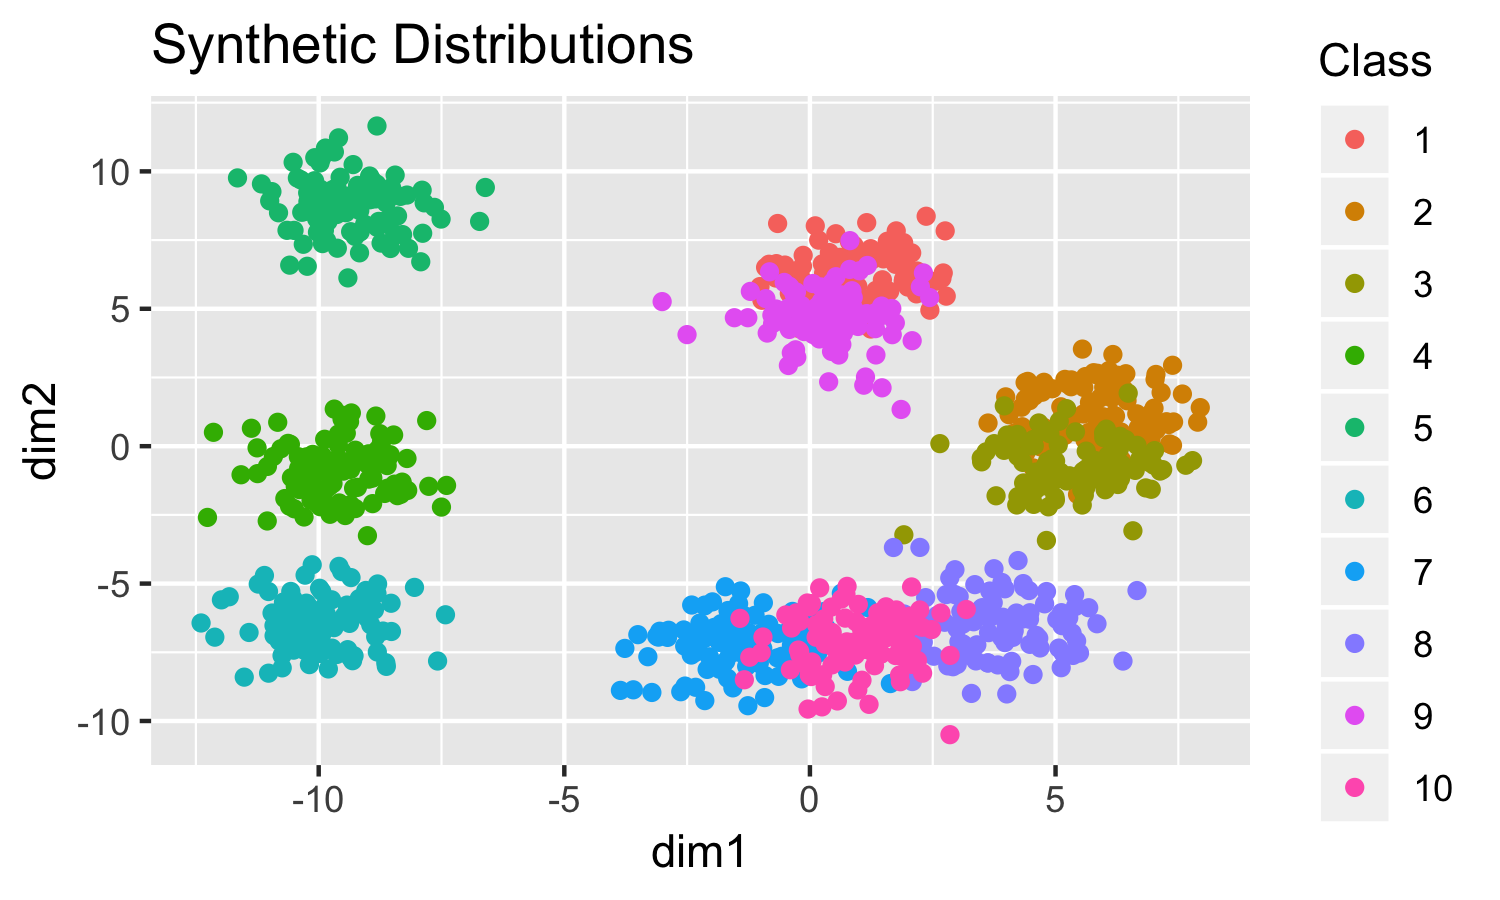
\includegraphics[width=\linewidth]{LabeledNormalPlot}
        \caption{Synthetic data.}
        \label{fig:synthetic_exp_1}
\end{subfigure}
\begin{subfigure}[b]{.5\textwidth}
\centering
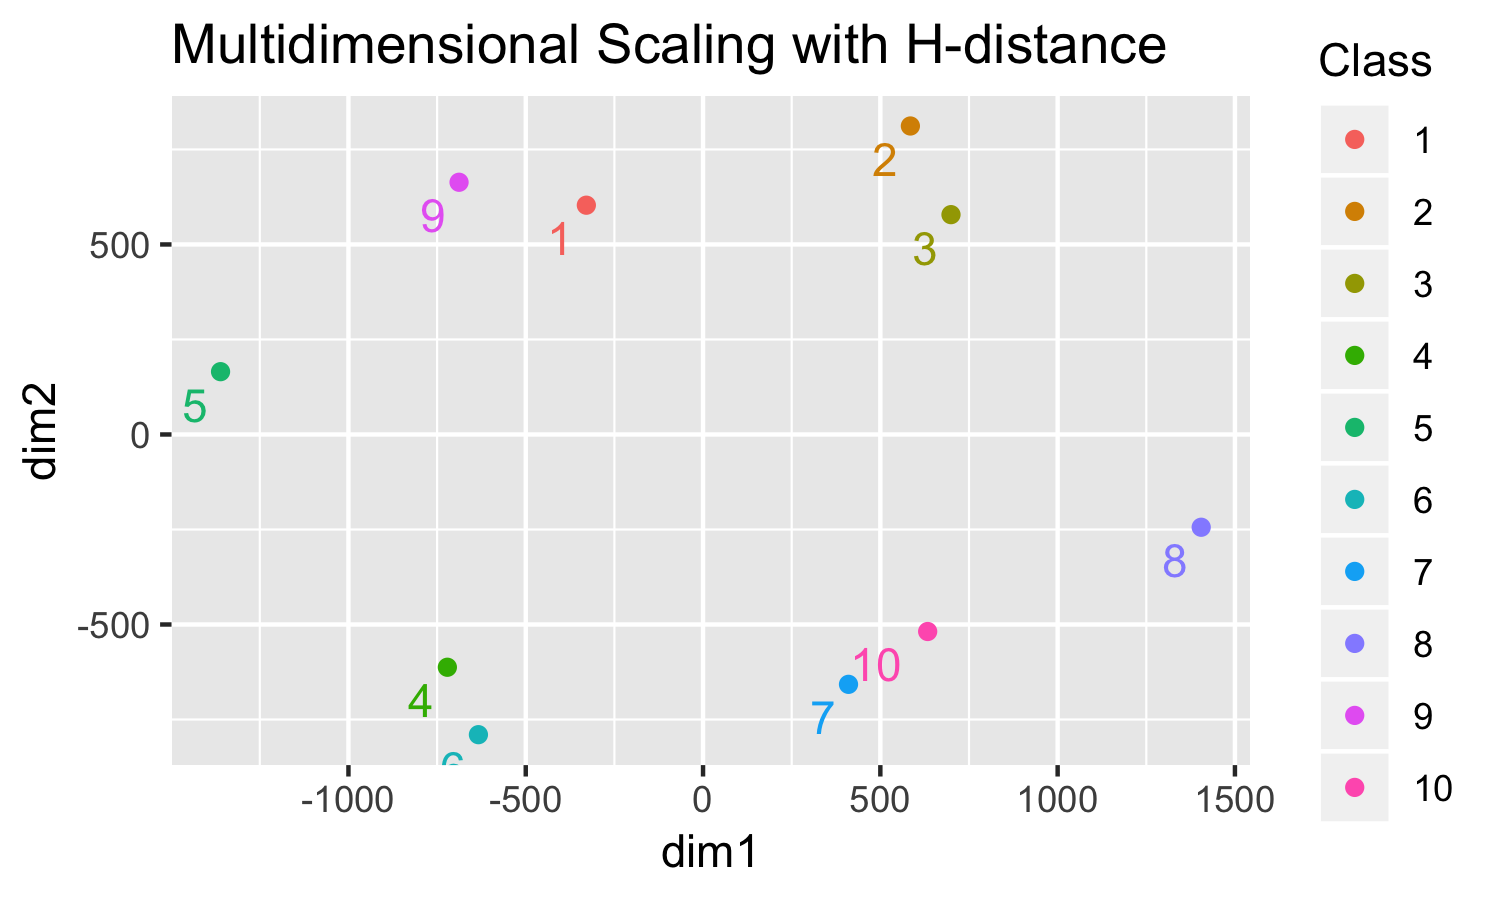
\includegraphics[width=\linewidth]{MDSNormalPlot}
        \caption{Multidimensional scaling with $H$-distance.}
        \label{fig:synthetic_exp_2}
\end{subfigure}
\caption{Hybrid Wasserstein distance for Gaussian data.}
\label{fig:synthetic_exp}
\end{figure}

As mentioned abov e, $T_X$ and $T_Y$ are not known and thus must be estimated. The following estimation procedure is recommended: Sample $X_1, ..., X_m \sim \tilde{P}_X$ and $R_1, ..., R_m \sim R$. Then find the optimal transport map, $\hat{T}_X$ from $\{X_i\}_{i=1}^m$ to $\{R_i\}_{i=1}^m$. For points outside of $\{X_i\}_{i=1}^m$, let $T_X$ map to the output of the 1-nearest neighbor.

\subsection{Complete Hybrid Wasserstein Distance}
Combining the results above with the closed form expression for the Wasserstein distance between two Gaussians, we get the complete expression for the sample hybrid Wasserstein distance:
\begin{equation}
\hat{H}^2(P_X, P_Y) = \| \hat{\mu}_X - \hat{\mu}_Y\|^2 + \mbox{tr}(\hat{\Sigma}_X) + \mbox{tr}(\hat{\Sigma}_Y) - 2\mbox{tr}((\hat{\Sigma}_X^{1/2} \hat{\Sigma}_Y \hat{\Sigma}_X^{1/2})^{1/2}) + \frac{1}{m} \sum\limits_{i=1}^m (\hat{T}_X(u_i) - \hat{T}_Y(u_i))^2
\end{equation}


\section{Experiments}\label{sec:experiments}
In this section, we perform two experiments to illustrate the utility of the hybrid wasserstein distance \footnote{Code can be found at \url{https://github.com/oconnor-kevin/clustering-with-ot}}.
\subsection{Synthetic Data}
First we apply the $H$-distance to a sample of Gaussian distributions in $\mathbb{R}^2$. $10$ means $\mu_1, ..., \mu_{10} \sim \mbox{Unif}[(-10, 10)^2]$ and $100$ points $x_{k,1}, ..., x_{k,100} \sim \mathcal{N}(\mu_k, \mathbf{I})$ for each $k = 1, ..., 10$ were generated and are depicted in Figure \ref{fig:synthetic_exp_1}. We then computed the $H$ distance between each pair of empirical distributions, $P_k$, where $P_k = 1/100  \sum_{i=1}^{100} \delta_{x_{k, i}}$, to obtain a matrix of pairwise $H$ distances. To visualize distances in this embedded space, we apply multi-dimensional scaling to obtain Figure \ref{fig:synthetic_exp_2}.  Note that the MDS plot mostly captures the relative centers of each distribution. This is to be expected as the true underlying distributions differ only in their means. Furthermore, for Gaussian distributions, $H$-distance reduces to the $W_2$ distance which is simply the Euclidean distance between the means for distributions with equal covariance.

\subsection{NBA Playoff Data}

\begin{figure}[t]
\centering
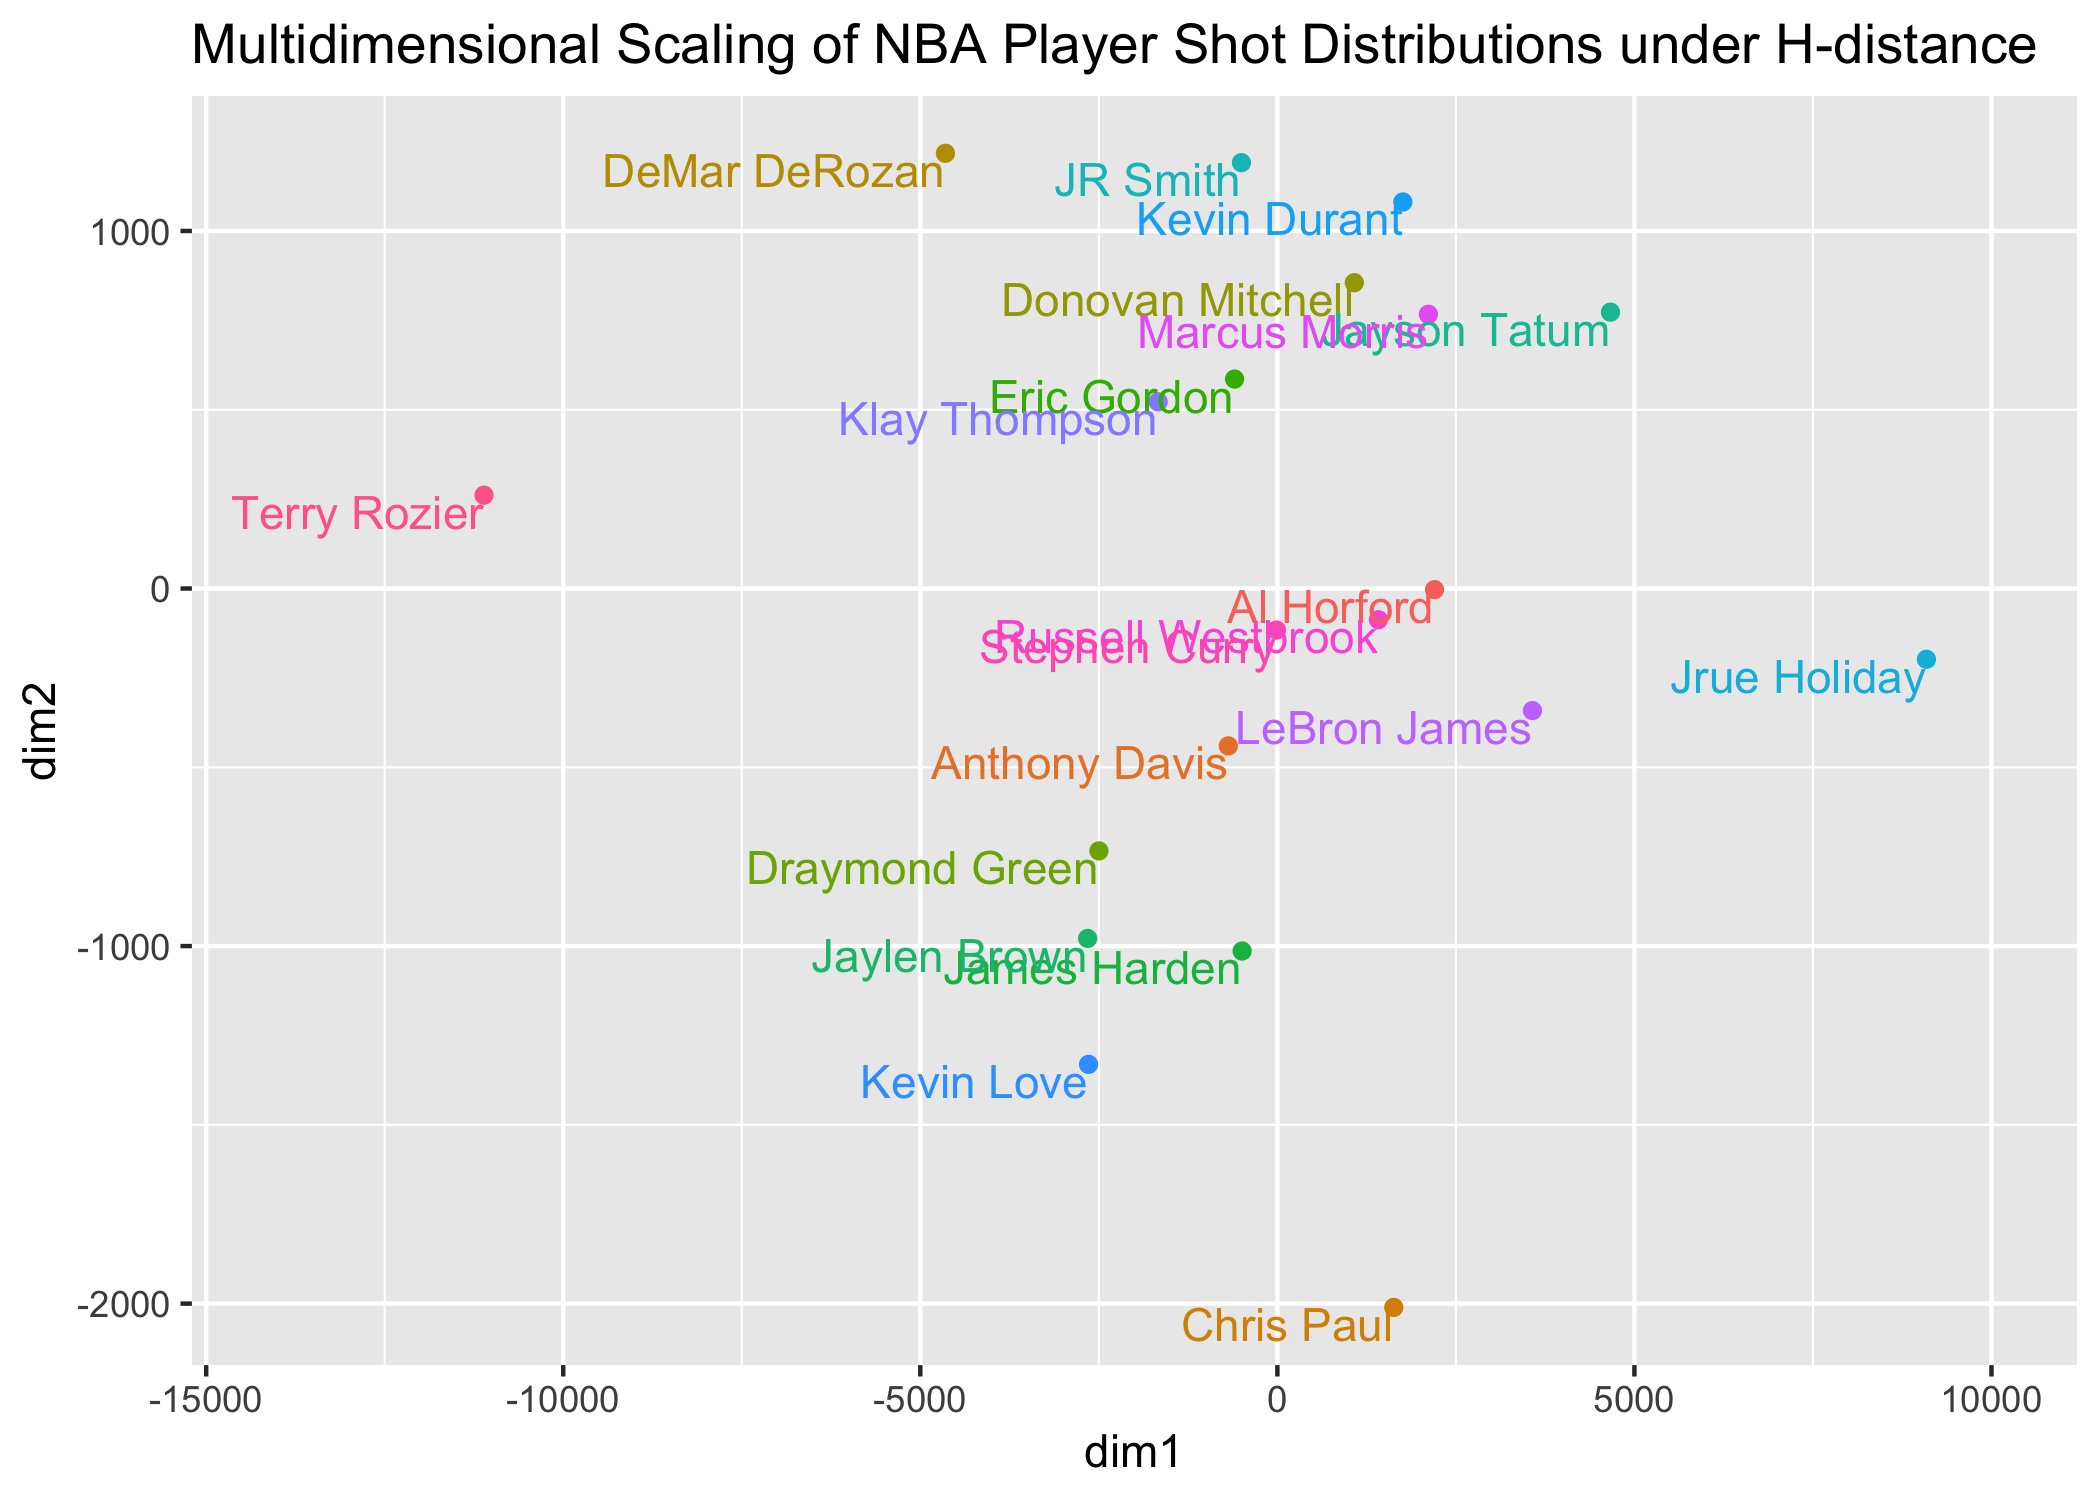
\includegraphics[width=\linewidth]{NBAMDSPlot}
\caption{Multidimensional scaling plot of NBA player shot distributions.}
\label{fig:nba}
\end{figure}


To investigate the effect of Hybrid Wasserstein distance on real data, we considered the distribution of made shots in the 2018 NBA playoffs \footnote{https://www.kaggle.com/boonpalipatana/nba-playoff-shots-2018}. This data contains the details of each shot taken by players in the 2018 NBA playoffs including coordinates of the shot and whether it went in or not. We can think of each player's made shots as comprising a distribution of court positions that we hope characterizes some aspect of their shooting style. We can then apply the Hybrid Wasserstein distance to compare players and use MDS to visualize the embedded space as above.

In order to make the data more digestible, we subset to players with more than 150 made shots in this dataset. The Hybrid Wasserstein distance matrix was computed between each player and used as input for MDS as above. The results are included in Figure \ref{fig:nba}. 

\section{Conclusion and Discussion}\label{sec:discussion}
We have seen how optimal transport defines a distance between distributions through the expectation of some ground metric. Furthermore, we have shown how to define a more efficient hybrid Wasserstein distance. Using this distance, we observed that distances between Gaussian data with equal covariances largely depend on the respective means. Finally, we demonstrated how one can measure distances between shot distributions of basketball players and use MDS to visualize the relationships between each.

There are many open questions regarding Wasserstein-based clustering methods. For example, what happens to Wasserstein-based clustering methods in high dimensions? In the case of the Hybrid Wasserstein distance, we expect that $\hat{\Sigma}$ will be a poor estimate of $\Sigma$ for high-dimensional data. It would be interesting to consider how this may affect clustering methods which leverage the $H$-distance. More generally, one could study what kinds of pathologies for distributions might cause outliers in Wasserstein-based distances and clustering. Then one may construct more robust distances with these pathologies in mind. A simple modification might be to use medians instead of means. Finally, what are the asymptotic distributional properties of the hybrid Wasserstein distance? Few results exist in this area for $W_2$ distance without Gaussian assumptions on the two distributions in question. One might try to find special cases where something can be said for the hybrid distance too.


\bibliographystyle{plain}
\bibliography{references}

\end{document}